\documentclass[0-thesis.tex]{subfiles}

\begin{document}
This chapter will analyze the proposed architecture qualitatively from the SUIT
specification as well as quantitatively evaluate the prototype, measuring energy
consumption, communication overhead, and code size.

\section{Qualitative Evaluation of Update Architecture}
\label{sec:qual-evaluation}
The proposed architecture was evaluated in two parts analogous to how the SUIT working
group presented their work, namely architecture and information model. Using the
requirements of each document, a qualitative evaluation of the proposed architecture was
performed. The requirements were gathered from \parencite{suit-architecture,
suit-information-model}.

\subsection{Architecture}
\label{ssec:arch-evaluation}
The SUIT architecture document specified ten requirements that a suitable update
architecture should fulfill. Table~\ref{tab:architecture-evaluation} lists these with
their corresponding motivations from the viewpoint of the proposed architecture.

\begin{small}
\begin{longtable}[]{@{}ll@{}}
    \caption{The SUIT architecture requirements and motivations of their fulfillment.}
    \label{tab:architecture-evaluation}\\
    \toprule
    \begin{minipage}[b]{0.41\columnwidth}\raggedright\strut
    Requirement\strut
    \end{minipage} & \begin{minipage}[b]{0.53\columnwidth}\raggedright\strut
    Fulfillment\strut
    \end{minipage}\tabularnewline
    \midrule
    \endfirsthead
    \toprule
    \begin{minipage}[b]{0.41\columnwidth}\raggedright\strut
    Requirement\strut
    \end{minipage} & \begin{minipage}[b]{0.53\columnwidth}\raggedright\strut
    Fulfillment\strut
    \end{minipage}\tabularnewline
    \midrule
    \endhead
    \toprule
    \begin{minipage}[b]{0.41\columnwidth}\raggedright\strut
    Requirement\strut
    \end{minipage} & \begin{minipage}[b]{0.53\columnwidth}\raggedright\strut
    Fulfillment\strut
    \end{minipage}\tabularnewline
    \midrule
    \endhead
    \toprule
    \begin{minipage}[b]{0.41\columnwidth}\raggedright\strut
    Requirement\strut
    \end{minipage} & \begin{minipage}[b]{0.53\columnwidth}\raggedright\strut
    Fulfillment\strut
    \end{minipage}\tabularnewline
    \midrule
    \endhead

    \begin{minipage}[t]{0.41\columnwidth}\raggedright\strut
    Agnostic to how firmware images are distributed\strut
    \end{minipage} & \begin{minipage}[t]{0.53\columnwidth}\raggedright\strut
    No parts of the architecture assumes a specific suite of protocols or
    algorithms to ensure secure delivery of updates. The architecture does
    specify the usage of technologies such as certificates, asymmetric
    encryption, and authorization tokens, but these elements can be
    implemented in a wide variety of ways using different protocols,
    algorithms, and certificate/token types. The profiles provided in this
    thesis are examples of how the architecture can be instantiated.\strut
    \end{minipage}\tabularnewline
    \begin{minipage}[t]{0.41\columnwidth}\raggedright\strut
    Friendly to broadcast delivery\strut
    \end{minipage} & \begin{minipage}[t]{0.53\columnwidth}\raggedright\strut
    The architecture itself does not limit broadcast delivery, and through
    correct usage of the manifest, broadcasted updates will not be
    incorrectly installed by devices other than the intended recipients.
    Choice of technology can limit the usage of broadcasting, such as DTLS,
    but this is implementation-specific.\strut
    \end{minipage}\tabularnewline
    \begin{minipage}[t]{0.41\columnwidth}\raggedright\strut
    Use state-of-the-art security mechanisms\strut
    \end{minipage} & \begin{minipage}[t]{0.53\columnwidth}\raggedright\strut
    The architecture is based on asymmetric cryptography using certificates,
    as well as access authorization through whitelists and possibly tokens
    for fine-grained authorization. Choice of key algorithms and token types
    will affect the cryptographic strength of the system.\strut
    \end{minipage}\tabularnewline
    \begin{minipage}[t]{0.41\columnwidth}\raggedright\strut
    Rollback attacks must be prevented\strut
    \end{minipage} & \begin{minipage}[t]{0.53\columnwidth}\raggedright\strut
    By specifying a monotonically increasing sequence number in the
    manifest, devices can make sure they are installing fresh images.
    Manifests are signed through COSE which ensures authenticity. An
    attacker would not be able to modify a manifest and compute a
    valid signature.\strut
    \end{minipage}\tabularnewline
    \begin{minipage}[t]{0.41\columnwidth}\raggedright\strut
    High reliability\strut
    \end{minipage} & \begin{minipage}[t]{0.53\columnwidth}\raggedright\strut
    This is an implementation specific-requirement, however the storage
    element of the manifest aids in achieving safe storage of a new image.
    After a successful update, devices are to re-register at servers. Until 
    the re-registration has occurred, the update might be redistributed. 
    This means an interrupted update can be rectified.\strut
    \end{minipage}\tabularnewline
    \begin{minipage}[t]{0.41\columnwidth}\raggedright\strut
    Operate with a small bootloader\strut
    \end{minipage} & \begin{minipage}[t]{0.53\columnwidth}\raggedright\strut
    The thesis suggests storing an unencrypted image alongside its digest
    for the bootloader to be minimal, only needing support for calculating a
    SHA256 digest of the image at boot. All information about whether or not
    to perform the update is encoded in conditions in the manifest, and can
    be stored with small memory usage.\strut
    \end{minipage}\tabularnewline
    \begin{minipage}[t]{0.41\columnwidth}\raggedright\strut
    Small parsers\strut
    \end{minipage} & \begin{minipage}[t]{0.53\columnwidth}\raggedright\strut
    The manifest format used in the thesis is simple, complete, and
    extensible. Parsing it requires storing the key/value pairs in
    predefined structures, which is doable even with a very small
    parser.\strut
    \end{minipage}\tabularnewline
    \begin{minipage}[t]{0.41\columnwidth}\raggedright\strut
    Minimal impact on existing firmware formats\strut
    \end{minipage} & \begin{minipage}[t]{0.53\columnwidth}\raggedright\strut
    The architecture makes no assumptions about firmware formats. It is up
    to the implementer to ensure the images are prepared for updating and
    that the bootloader contains the necessary functionality. Transporting
    the images is the same regardless of content.\strut
    \end{minipage}\tabularnewline
    \begin{minipage}[t]{0.41\columnwidth}\raggedright\strut
    Robust permissions\strut
    \end{minipage} & \begin{minipage}[t]{0.53\columnwidth}\raggedright\strut
    The architecture is based on asymmetric cryptography using certificates
    for identity and confidentiality, and whitelists of servers and
    operators as possibly tokens for authorization. Different deployments
    have different security and performance requirements. The architecture
    is flexible by allowing different kinds of key algorithms, encryption
    schemes, and token types. Some deployments may not need tokens at all, as
    authentication is done on a device level and whitelists are sufficient,
    white other deployments wanting to update specific pieces of a device
    may need fine-grained authorization through tokens. Different devices in
    the same deployment can have different authorization configurations 
    (e.g., by accepting different types of tokens).\strut
    \end{minipage}\tabularnewline
    \begin{minipage}[t]{0.41\columnwidth}\raggedright\strut
    Operating modes\strut
    \end{minipage} & \begin{minipage}[t]{0.53\columnwidth}\raggedright\strut
    The architecture supports the device-initiated pull model as well as the
    operator-initiated push model. The update server acts as a mediator
    between device and operator as well as a repository for images and
    device profiles, letting the operator query the server for device
    statuses, and devices query for updates, depending on the model
    used.\strut
    \end{minipage}\tabularnewline
    \bottomrule
\end{longtable}
\end{small}
  
\subsection{Information Model}
\label{ssec:information-evaluation}
The information model had more requirements imposed on it than the architecture, and its
implementation forms an important basis for carrying out safe updates.
Table~\ref{tab:information-evaluation} lists the requirements for the information model
alongside their motivations.

\begin{small}
\begin{longtable}[]{@{}ll@{}}
    \caption{The SUIT requirements on the information model and motivations of their fulfillment.}
    \label{tab:information-evaluation}\\
    \toprule
    \begin{minipage}[b]{0.37\columnwidth}\raggedright\strut
    Requirement\strut
    \end{minipage} & \begin{minipage}[b]{0.57\columnwidth}\raggedright\strut
    Fulfillment\strut
    \end{minipage}\tabularnewline
    \midrule
    \endfirsthead
    \toprule
    \begin{minipage}[b]{0.37\columnwidth}\raggedright\strut
    Requirement\strut
    \end{minipage} & \begin{minipage}[b]{0.57\columnwidth}\raggedright\strut
    Fulfillment\strut
    \end{minipage}\tabularnewline
    \midrule
    \endhead

    \begin{minipage}[t]{0.37\columnwidth}\raggedright\strut
    Monotonic sequence numbers\strut
    \end{minipage} & \begin{minipage}[t]{0.57\columnwidth}\raggedright\strut
    The manifest contains monotonically increasing sequence numbers to
    prevent rollback attacks to older version of firmware. Signed manifests
    ensure an attacker cannot modify an old manifest to update the
    sequence number and roll back the device firmware.\strut
    \end{minipage}\tabularnewline
    \begin{minipage}[t]{0.37\columnwidth}\raggedright\strut
    Vendor and device-type identifiers\strut
    \end{minipage} & \begin{minipage}[t]{0.57\columnwidth}\raggedright\strut
    This thesis used nested UUID5 identifiers as vendor and device
    identifiers where the vendor UUID is the namespace for the device UUID.
    These are implemented as preconditions in the manifest format.\strut
    \end{minipage}\tabularnewline
    \begin{minipage}[t]{0.37\columnwidth}\raggedright\strut
    Best-before timestamps\strut
    \end{minipage} & \begin{minipage}[t]{0.57\columnwidth}\raggedright\strut
    This can be added as an option or precondition.\strut
    \end{minipage}\tabularnewline
    \begin{minipage}[t]{0.37\columnwidth}\raggedright\strut
    Cryptographic authenticity\strut
    \end{minipage} & \begin{minipage}[t]{0.57\columnwidth}\raggedright\strut
    Payloads are signed in COSE which ensures authenticity. The image digest
    is also calculated and checked against the digest in the manifest.\strut
    \end{minipage}\tabularnewline
    \begin{minipage}[t]{0.37\columnwidth}\raggedright\strut
    Authenticated payload type\strut
    \end{minipage} & \begin{minipage}[t]{0.57\columnwidth}\raggedright\strut
    The payload format is mandatory, carried in the signed manifest.\strut
    \end{minipage}\tabularnewline
    \begin{minipage}[t]{0.37\columnwidth}\raggedright\strut
    Authenticated storage location\strut
    \end{minipage} & \begin{minipage}[t]{0.57\columnwidth}\raggedright\strut
    The storage location is mandatory, carried in the signed manifest.\strut
    \end{minipage}\tabularnewline
    \begin{minipage}[t]{0.37\columnwidth}\raggedright\strut
    Authenticated remote resource location\strut
    \end{minipage} & \begin{minipage}[t]{0.57\columnwidth}\raggedright\strut
    The URL is mandatory in the payloadInfo structure carried in the signed
    manifest.\strut
    \end{minipage}\tabularnewline
    \begin{minipage}[t]{0.37\columnwidth}\raggedright\strut
    Secure boot\strut
    \end{minipage} & \begin{minipage}[t]{0.57\columnwidth}\raggedright\strut
    Information enabling secure boot such as image digest and size is
    included in the signed manifest.\strut
    \end{minipage}\tabularnewline
    \begin{minipage}[t]{0.37\columnwidth}\raggedright\strut
    Authenticated precursor images\strut
    \end{minipage} & \begin{minipage}[t]{0.57\columnwidth}\raggedright\strut
    All precursors must have their URLs and digests included in the signed
    manifest.\strut
    \end{minipage}\tabularnewline
    \begin{minipage}[t]{0.37\columnwidth}\raggedright\strut
    Authenticated vendor and class IDs\strut
    \end{minipage} & \begin{minipage}[t]{0.57\columnwidth}\raggedright\strut
    These are both are implemented as preconditions in the signed manifest.\strut
    \end{minipage}\tabularnewline
    \begin{minipage}[t]{0.37\columnwidth}\raggedright\strut
    Rights require authenticity\strut
    \end{minipage} & \begin{minipage}[t]{0.57\columnwidth}\raggedright\strut
    Exercising different rights can be achieved through the use of
    certificates (identity), whitelists (coarse-grain access control), and
    tokens (fine-grain access control).\strut
    \end{minipage}\tabularnewline
    \begin{minipage}[t]{0.37\columnwidth}\raggedright\strut
    Firmware encryption\strut
    \end{minipage} & \begin{minipage}[t]{0.57\columnwidth}\raggedright\strut
    All communication in the architecture is encrypted and the payloads are
    signed. Keys for encryption are handled through certificates and for
    signing through the content key method manifest element.\strut
    \end{minipage}\tabularnewline
    \begin{minipage}[t]{0.37\columnwidth}\raggedright\strut
    Access control lists\strut
    \end{minipage} & \begin{minipage}[t]{0.57\columnwidth}\raggedright\strut
    Access control is achieved through whitelists of operators and update
    servers and possibly tokens.\strut
    \end{minipage}\tabularnewline
    \begin{minipage}[t]{0.37\columnwidth}\raggedright\strut
    Encrypted manifests\strut
    \end{minipage} & \begin{minipage}[t]{0.57\columnwidth}\raggedright\strut
    All communication in the architecture is encrypted and signed.\strut
    \end{minipage}\tabularnewline
    \bottomrule
\end{longtable}
\end{small}

\section{Quantitative Evaluation of Update Architecture}
\label{sec:quant-evaluation}
This section presents the results of an experiment carried out to measure the energy
consumption of the prototype on Firefly boards, described in
Section~\ref{ssec:experimental-setup}. In addition to energy consumption, code size and
communication overhead are also reported. 

\subsection{Energy Consumption}
\label{ssec:energy-consumption}

Figures \ref{fig:client-operations-energy} and \ref{fig:server-operations-energy} show
average energy consumption for registration-and manifest-related operations for the client
and server. Figures \ref{fig:client-image-energy} and \ref{fig:server-image-energy} shows
average energy consumption for the client and server when encrypting, transferring, and
decrypting image data per block size. Standard deviations are included as error bars for
all measurements, but in most cases are too small to be visible.

\begin{figure}[]
    \caption{Average energy consumption for client operations.}
    \label{fig:client-operations-energy}
    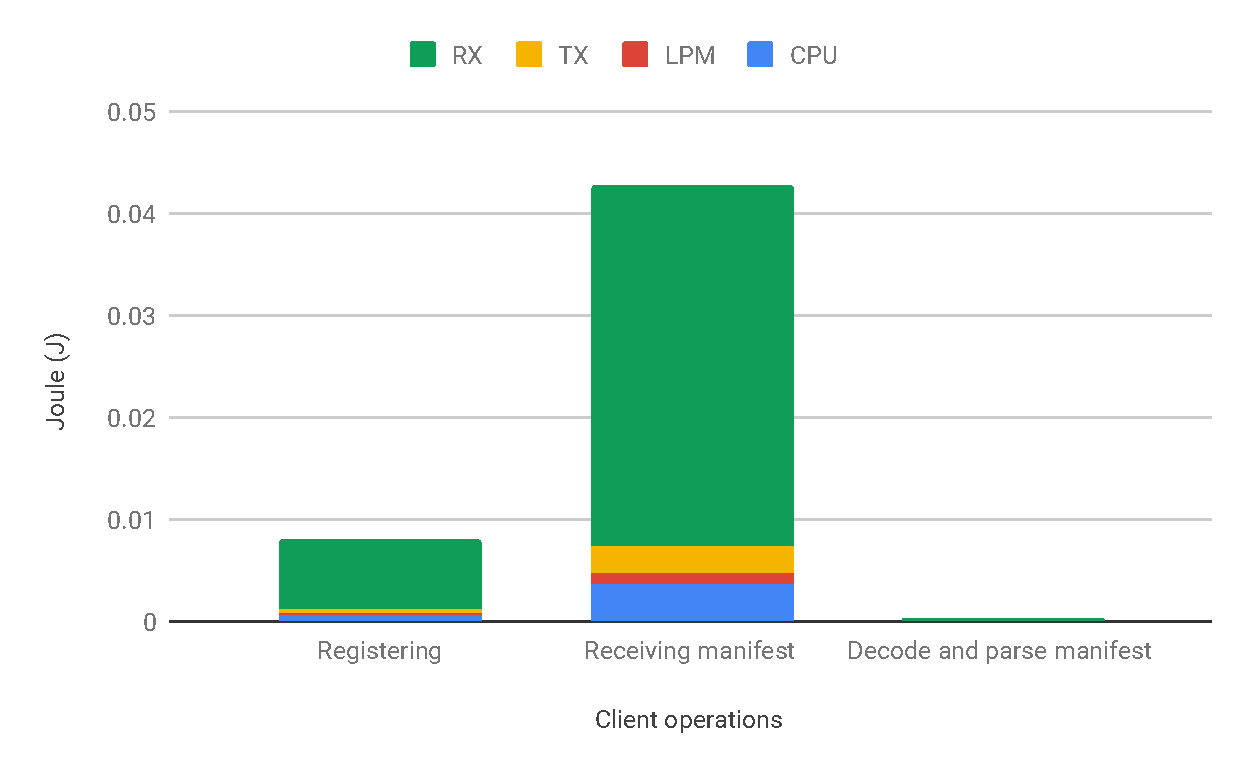
\includegraphics[scale=0.77]{images/client-operations-energy.pdf}
\end{figure}

\begin{figure}[]
    \caption{Average energy consumption for server operations.}
    \label{fig:server-operations-energy}
    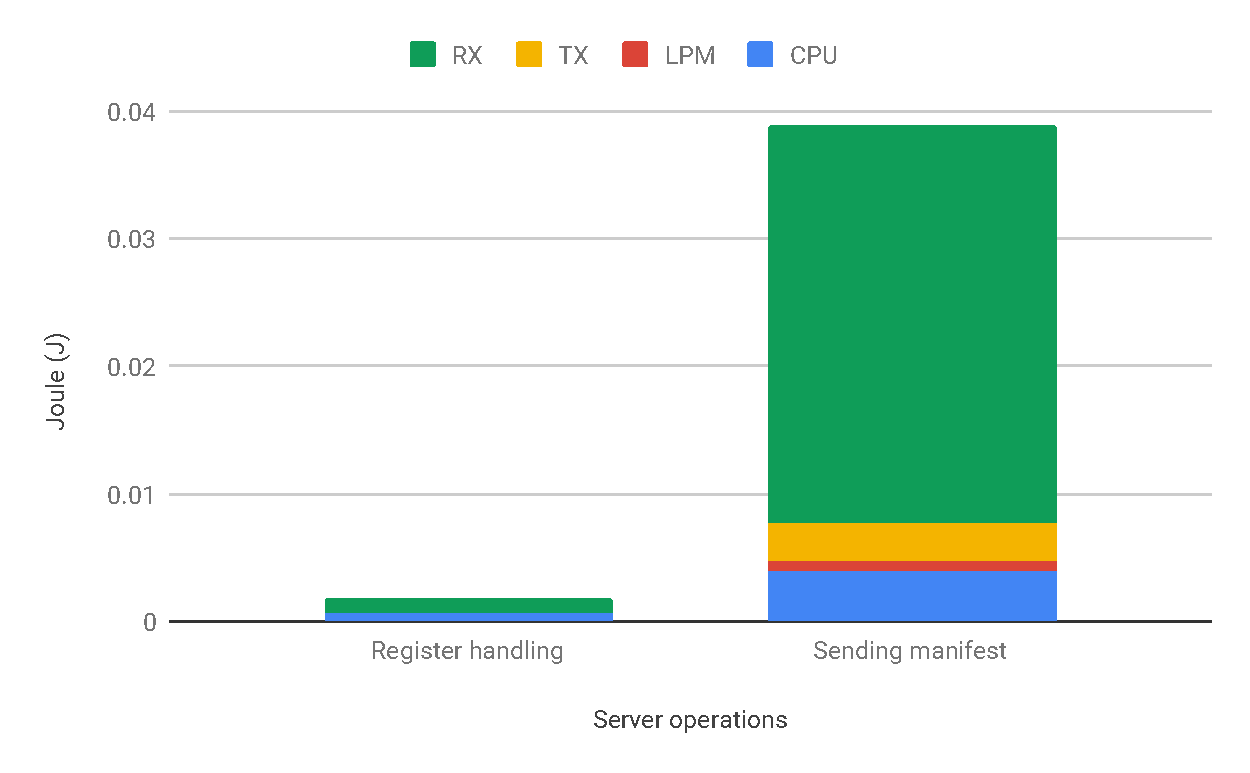
\includegraphics[scale=0.77]{images/server-operations-energy.pdf}
\end{figure}

\begin{figure}[]
    \caption{Average energy consumption for client during image transfer.}
    \label{fig:client-image-energy}
    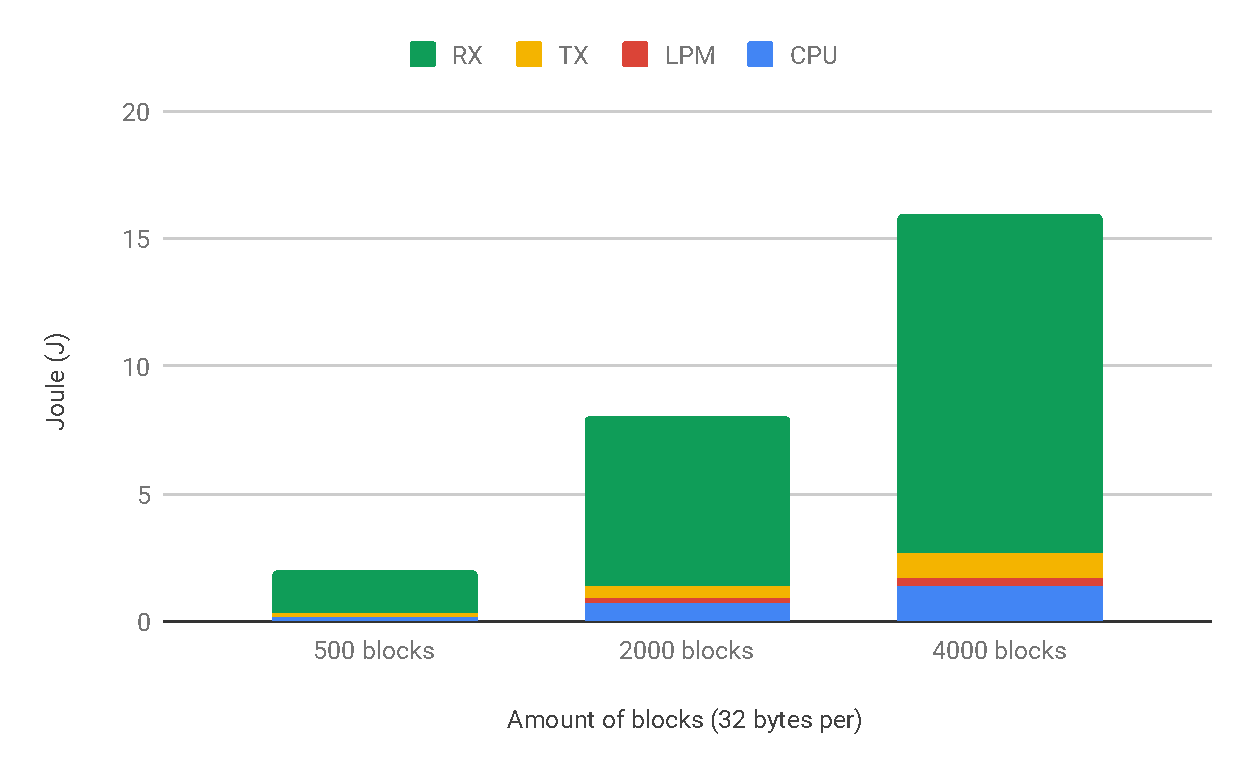
\includegraphics[scale=0.77]{images/client-image-energy.pdf}
\end{figure}

\begin{figure}[]
    \caption{Average energy consumption for server during image transfer.}
    \label{fig:server-image-energy}
    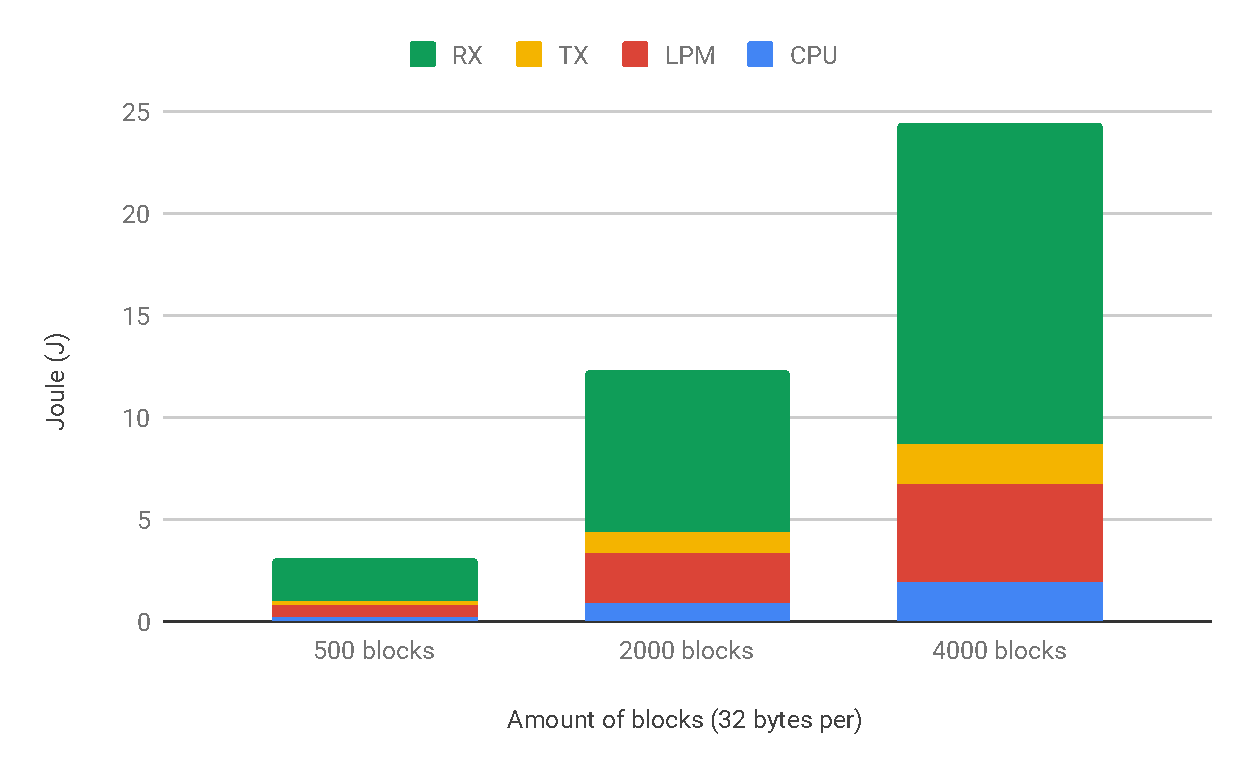
\includegraphics[scale=0.77]{images/server-image-energy.pdf}
\end{figure}

\newpage    % Force new page so previous graphs appear in order
\subsection{Communication Overhead}
\label{ssec:communication-overhead}
As discussed in Section~\ref{ssec:prototype-implementation}, some overhead is introduced
at the application layer as a consequence of using COSE encryption. Each CoAP block sent by
the server during image transfer contains 32 bytes of data, of which 8 is a tag used to
validate the ciphertext. Figure~\ref{fig:communication-overhead} shows this disparity.

\begin{figure}[t]
    \caption{Bytes transferred vs actual data sent measured in bytes at the application layer.}
    \label{fig:communication-overhead}
    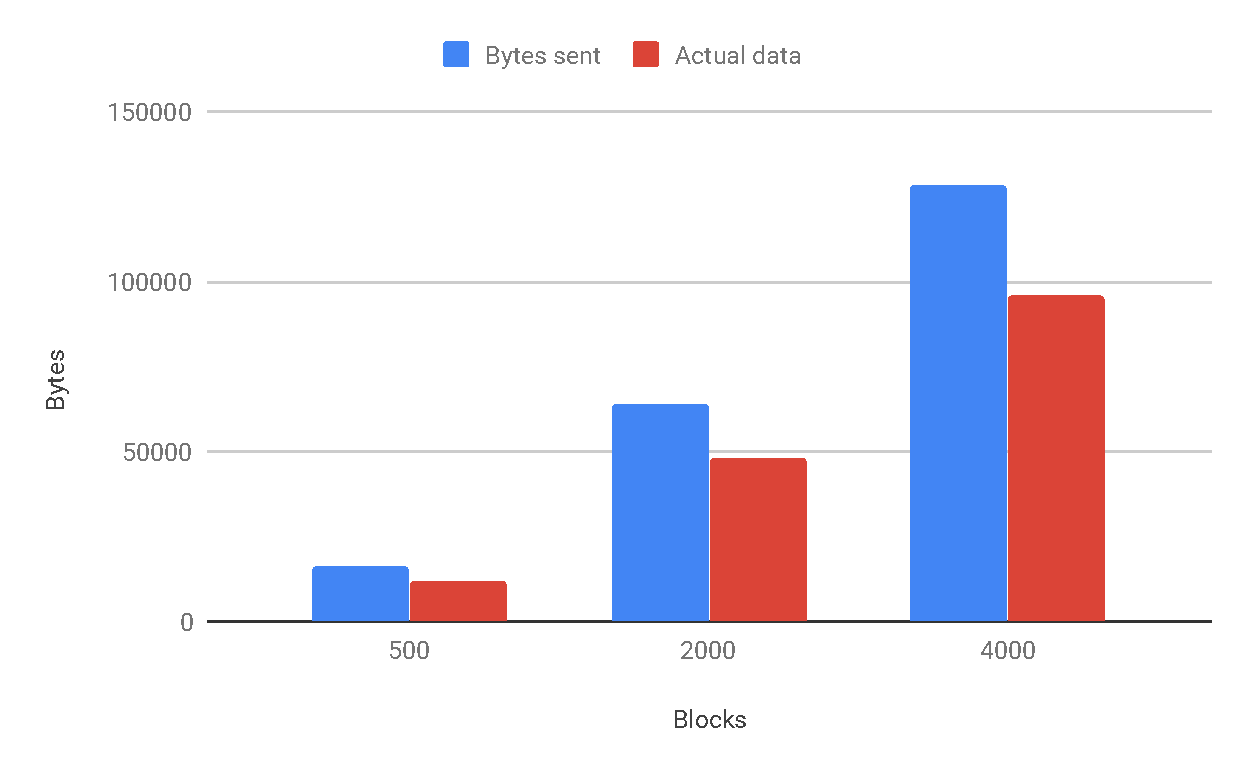
\includegraphics[scale=0.65]{images/communication-overhead.pdf}
\end{figure}

\subsection{Code Size}
\label{ssec:code-size}
When measuring code size, the code was compiled with all debug macros set to 0, the
energest measurements removed, and no other Contiki-NG modules included except CoAP. As a
point of reference, a bare-bones example was also created. The bare-bones example only
contains the necessary imports to Contiki-NG and its CoAP engine and declares a process
with no code in it. It is the smallest runnable example for Firefly devices using the same
project configuration as the other source files. Its source code is found in
Appendix~\ref{app:bare-bones}. By running the tool \texttt{arm-none-eabi-size} on the
ELF-files the code size can be obtained, which is shown in Table~\ref{tab:code-size}.

\begin{table}[!t]
\begin{tabular}{l c r r r l}
text	&  data	 &  bss	 &  dec	 &  hex&filename\\
69982	&  1772	 &11303	 &83057	 &14472&bare-bones.elf\\
75956	&  1788	 &13599	 &91343	 &164cf&update-client.elf\\
77924	&  1884	 &11835	 &91643	 &165fb&update-server.elf
\end{tabular}
\caption{Code size for client and server prototypes.}
\label{tab:code-size}
\end{table}

\end{document}